\documentclass{article}
\usepackage[utf8]{inputenc}

\usepackage{amsmath} % package for adding equations
\usepackage{graphicx} % package for adding images
\usepackage[hidelinks]{hyperref}
\usepackage{parskip} % package for adding new lines
\usepackage{pythonhighlight} % package for writing python code
\usepackage{tabularx} % package for creating tables
\usepackage{subcaption} % allows having two images side by side

\graphicspath{ {figs/} }

\title{Forecast the popularity of SearX with epidemiological models}
\author{Rita Ferrolho }
\date{July 2021}

\begin{document}
\maketitle % the whole preambule (cover page) is printed here
\tableofcontents % index table is generated here

\section*{Introductory Note}
\addcontentsline{toc}{section}{Unnumbered Section} % adds unnumbered section to table of contents
This document presents an approach overview of SearX, a metasearch engine. It is a continuation of a previous assignment [1], however, a deeper analysis of the epidemiological models, in the context of information technologies, will be made. Particularly, more models will be discussed, simulations of those models will be presented and more advanced topics will be explored, such as the Gillespie algorithm and optimal control. A deeper analysis of churn will also be made. Despite the discussion of these new topics, some of the previous work will be shown in this report.


% chapters and sections 

\section{Abstract} % TODO: add citations for bibliography
SearX is a non-profit, privacy-respecting metasearch engine which was initially released in 2014, by Adam Tauber. Unlike most private engines, SearX is open-source [2]. This means that any developer can analyze the code and make their own conclusions regarding its privacy. The engine can be used by choosing one of the SearX-instances available online [3]. If the user isn’t comfortable using any of those instances, they can install the software [4]. Further details about this engine can be found in its documentation [5].

\section{Metasearch and Crawler Engines}
In order to be familiar with the mechanism behind SearX’s engine, it is important to learn the difference between a metasearch engine and a regular search engine.

Metasearch engines, as shown in \autoref{fig:metasearch}, are engines which use results from other search engines in order to get it’s own results which are constructed by aggregating and ranking the results of other search engines. These are usually faster and provide a wider net of results.

\begin{figure}[ht]
    \centering
    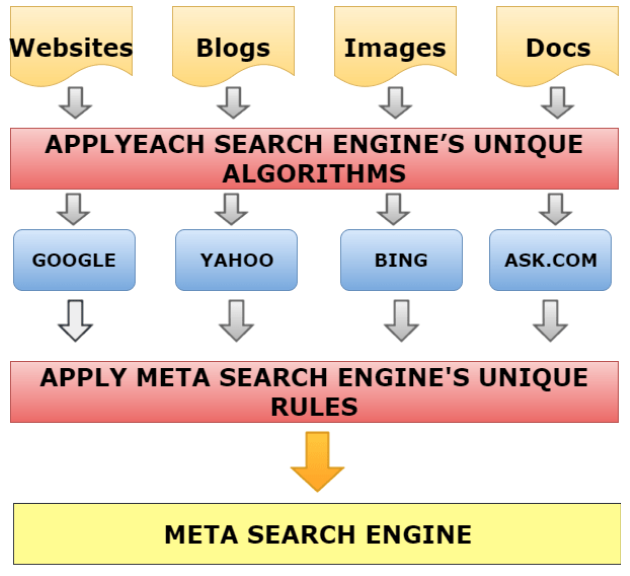
\includegraphics[width=0.5\linewidth]{metasearch}
    \caption{Metasearch engine diagram.}
    \label{fig:metasearch}
\end{figure}

On the other hand, a search engine, also known as a crawler engine, is a software system that is designed to perform web searches, which means to search the world wide web systematically, aiming to find the requested query. The search results are presented to the users and are often referred to as search engine pages. Those pages are known as SERPS - Search Engine Results Pages [6].

\autoref{fig:meta_vs_crawler} may be useful in understanding the differences between those engines.

\newpage

\begin{figure}[h]
    \centering
    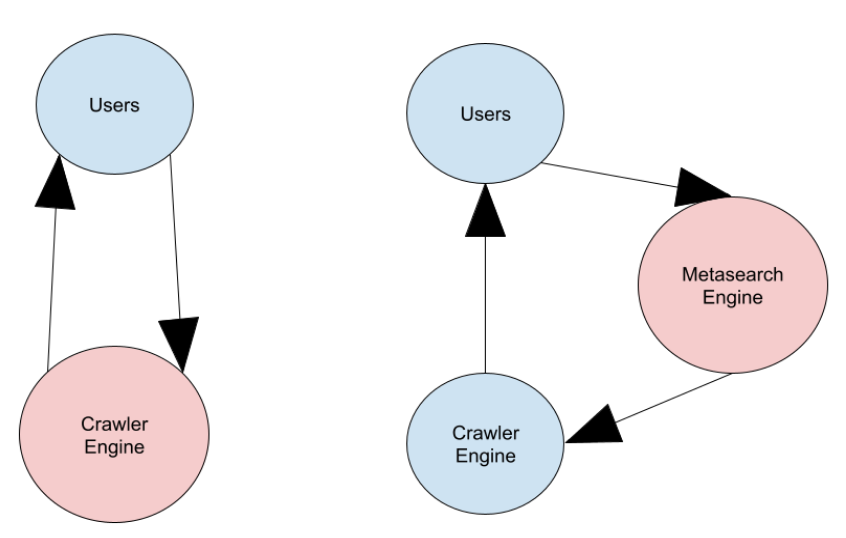
\includegraphics[width=0.7\linewidth]{meta_vs_crawler}
    \caption{Difference between a crawler engine, represented on the diagram from the left, and a metasearch engine, represented on the diagram from the right.}
    \label{fig:meta_vs_crawler}
\end{figure}


\section{SearX Algorithm}
The algorithm used by SearX to show its query results is represented in the function below:

\begin{python}
def result_score(result):
    weight = 1.0

    for result_engine in result['engines']:
        if hasattr(engines[result_engine], 'weight'):
            weight *= float(engines[result_engine].weight)

    occurrences = len(result['positions'])

    return sum((occurrences * weight) / position for position in result['positions'])
\end{python}


% TODO: write code in python format
Every result gets a score calculated by sum((occurrences × weight) / position for position in result['positions']), where occurrences is the number of engines searched that recommended this result, weight is the product of the weights assigned to every regular search engine where this result appeared, by default every active search engine has this value set to 1. For each instance of this result, the aforementioned product is divided by the position it held in the recommendation list of each of the regular engines which have recommended it, so results with higher priority in other search engines will develop a higher ranking in SearX.

The sum of this value calculated for every instance of this results appearance in the regular engines SearX searched gives us the result’s priority.

By translating this algorithm to the mathematical language, the following formula can be obtained:

\begin{equation} % TODO: fix second sum in the equation
    \text{Result Score} = \sum_\text{position}^\text{positions} \frac{(\sum_\text{position}^\text{positions} 1) * (\sum_\text{engine}^\text{engines} \text{weight}_\text{engine})}{\text{position}} 
\end{equation}

This is a simple yet effective method of aggregating the priority of a result throughout multiple search engines. Which search engines are active in the search and which priority each one holds can be customized through properties directly in the settings.yml, a file that is included in the source code. At the moment, there isn’t a user-friendly way to customize these options.

\section{Modeling and Simulation of the popularity of SearX}

One of the main goals of this assignment is to forecast the popularity of SearX. A more concrete goal can be defined as the following:

\begin{center}
    \textit{Forecast the evolution of SearX’s popularity in Portugal, between 2014 and 2050.}
\end{center}

There are several mathematical models [7] that can help us to achieve this goal. The study of epidemiological models, for instance, can be very helpful in this work, since these models can be adapted to other contexts, even in the field of information technologies. 

When developing a model, it is necessary to model the x axis, y axis, functions and initial conditions, at least. Given the goal written above, to model the x axis, it can be deducted that $\Delta t = [2014, 2050]$, which will correspond to the x axis, where the time interval between $t_x$ and $t_x+1$ is approximately a month. There will be one exception in this report, however, in the Gillespie algorithm, since it requires a different approach to determine $\Delta t$, which cannot be entirely controlled by the programmer, as it will be later discussed.

The y axis will be modelled for the range $[0, N]$, where Nis the population which will be applied in the model. At first, it might seem obvious that the value of Nwill correspond to the whole portuguese population, that is, $N = 10 166 984$ [8], but depending on the factors being considered, the value of Nmight be lower. For instance, if only the people with access to the internet are taken into consideration, a suggestive value for $N$ would be $N = 10 166 984 * 0.76 = 7 726 907$ [9]. Besides, some models may require a lower value of N in order to execute the simulation effectively, in which case it is preferable to use $N = 1000$. At last, but not least, the functions of the model can be modeled in vastly different ways, depending on how the problem is being interpreted. These functions will soon be discussed in further detail, as well as the initial conditions.

It is unfortunate to mention that no datasets regarding the popularity of the engine were found, so the models were developed without taking any real data into consideration. This is also the reason why it has been decided to create the models for a time range that includes years prior to the current year, by beginning from the year when SearX was first launched.

\subsection{SI Model}

A SI Model, which stands for Susceptible (S) and Infectious (I), is an epidemiological model which estimates the number of people contaminated with a contagious disease, in a closed population and over time. The total population is represented by N, defined by N = S(t)+I(t) = 7 726 907. By the way, for any epidemiological model presented in this work, the value of N will always correspond to the sum of all the functions involved in the model (excluding the optimal control), meaning that $\sum_k^K S_k(t)$, where K is the total number of functions, k specifies the function and $S_k(t)$ is the function itself. 

The diagram shown in \autoref{fig:SI} is a visual representation of the SI model.

\begin{figure}[h]
    \centering
    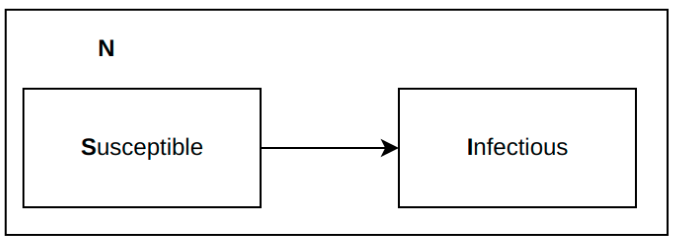
\includegraphics[width=0.5\linewidth]{SI}
    \caption{SI model diagram.}
    \label{fig:SI}
\end{figure}

In the context of SearX, the interpretation of the SI model could be made according to \autoref{fig:SI2}.

\begin{figure}[h]
    \centering
    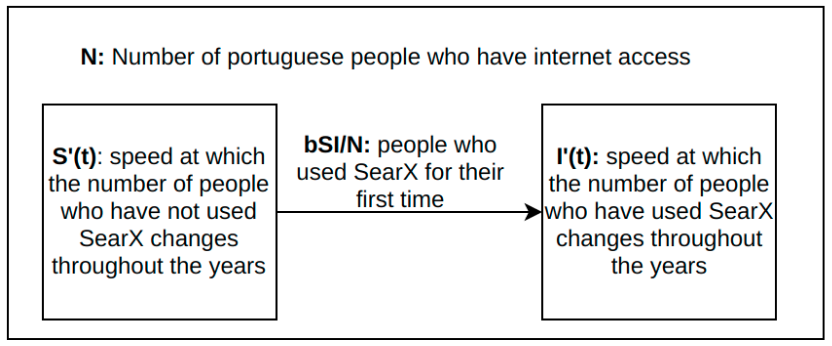
\includegraphics[width=0.5\linewidth]{SI2}
    \caption{SI model diagram, adapted to the context of SearX.}
    \label{fig:SI2}
\end{figure} 

The model shown at \autoref{fig:SI2} is likely to raise some questions for those who are unfamiliar with the model, including:

\begin{enumerate}
    \item What is the meaning of S(t) and I(t)? 
    \item What are the initial conditions?
    \item What parameters are represented in $\frac{bSI}{N}$ and why?
    \item Why are the S’(t) and I’(t) functions being modeled instead of S(t) and I(t)?
\end{enumerate}

The answer for the question (1) is presented in the table below:

\begin{tabularx}{1\textwidth} { 
    | >{\centering\arraybackslash}X 
    || >{\centering\arraybackslash}X | }
   \hline
   S(t) & Number of people who have not used SearX in time t. \\
   \hline
   I(t)  & Number of people who have used SearX in time t. \\
  \hline
\end{tabularx}

As for the question (2), the initial conditions are formally known as S(2014) and I(2014), since the initial value of t is $t_0 = 2014$. Assuming that only one person has used SearX, that is, only one person is from the Infectious group, the initial conditions are the following:

\[ S(2014) = N - I(2014) = 7 726 907-1= 7 726 906 \]
\[ I(2014) = 1 \]

As for the question (3), b corresponds to the ratio of people, from the Susceptible group, who transition to the Infectious group, that is, who use SearX for their first time. This value is then multiplied by S, bS, to get the number of people moving from the Susceptible group to the Infectious group. Then, bS is multiplied by I, bSI, because the people represented by I have an influence on a certain number of people from the Susceptible group, convincing them to become part of the Infectious group. For example, if marketing strategies are implemented for SearX, the engine is more likely to be popular than if no marketing strategies are made, as more people will notice the engine and use it. Last, but not least, since $N>1$, it is necessary to divide the expression by N, $\frac{bSI}{N}$. By the way, $\frac{b}{N}$ could be interpreted as the probability of someone using SearX for their first time.

With all the necessary states and transitions established, it is now possible to formally describe the model by a set of ordinary differential equations (ODEs), as written below. There is only one transition going from the Susceptible group to the Infectious group, as presented in \autoref{fig:SI2}, therefore $\frac{dS}{dt} <= 0$, $\frac{dI}{dt} >= 0$ and $\frac{dI}{dt} = - \frac{dI}{dt}$.

\[ \frac{dS}{dt} = - \frac{bSI}{N} \]
\[ \frac{dI}{dt} = \frac{bSI}{N}  \]

An analysis of these ODEs suggests that the higher the value of b, the lower the value of S’(t) and the higher the value of I’(t). This means that S(t) will decrease faster and I(t) will grow more quickly. Consequently, the popularity of SearX will have a faster improvement. This conclusion can be confirmed by basic plots that represent the results of the simulation of this model.

Lastly, as for the question (4), the ODEs are included in the model instead of their integrals, S(t) and I(t), because, in the implementation, those integrals will be later determined by using the odeint module [10], particularly the LSODA package [11]. Besides, differential equations, including ODEs, are typically used to model the behavior of complex systems, such as dynamic systems [12]. A dynamic system is a system that is constantly changing, with an output that is dependent on time. Dynamic systems also tend to become static or reach a state of equilibrium over time [13]. The SI model is an example of such a system.

Since the model is complete, the simulations can be made, as shown in \autoref{fig:plts1_SI1} and \autoref{fig:plts1_SI2}. These simulations were based on the code presented in a blog maintained by Christian Hill [14].

\begin{figure}[h]
    \centering
    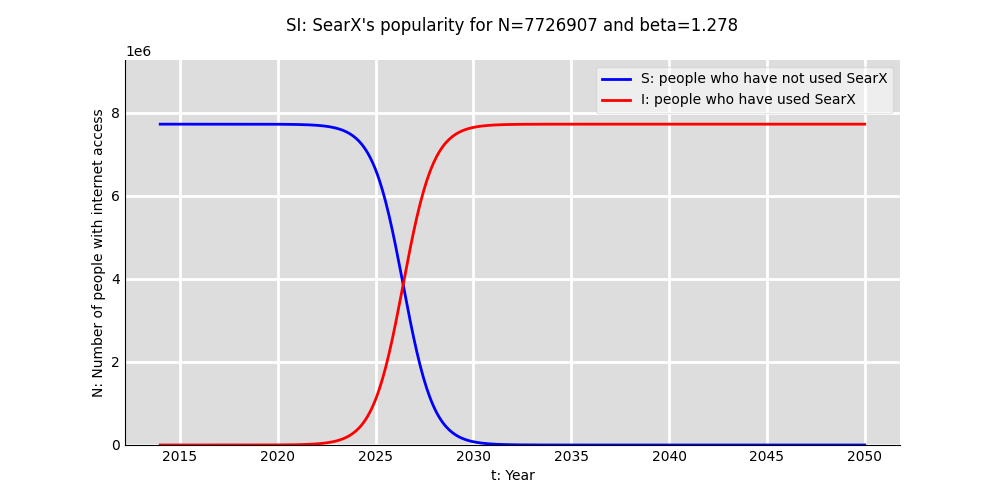
\includegraphics[width=0.8\linewidth]{plts1_SI1}
    \caption{Simulations‌ ‌of‌ ‌the‌ ‌adapted‌ ‌SI‌ ‌model,‌ ‌for‌ b = 1.278.}
    \label{fig:plts1_SI1}
\end{figure}

\begin{figure}[h]
    \centering
    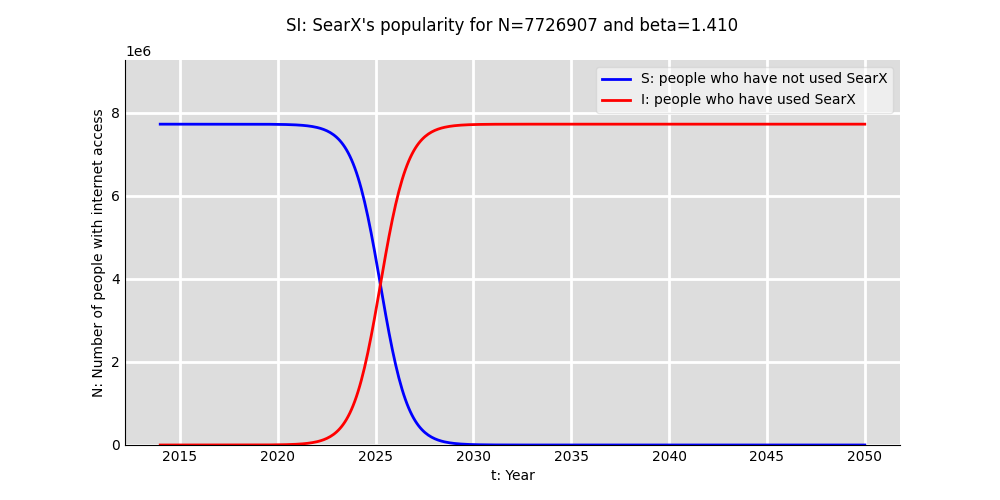
\includegraphics[width=0.8\linewidth]{plts1_SI2}
    \caption{Simulations‌ ‌of‌ ‌the‌ ‌adapted‌ ‌SI‌ ‌model,‌ ‌for‌ ‌b = 1.410.‌}
    \label{fig:plts1_SI2}
\end{figure}

The‌ ‌simulations‌ ‌confirm‌ ‌that‌ ‌if‌ ‌the‌ ‌value‌ ‌of‌ ‌\emph{b‌} ‌is‌ ‌increased,‌ ‌the‌ ‌popularity‌ ‌of‌ ‌SearX‌ ‌has‌ ‌a‌ ‌quicker‌‌ improvement.‌

\subsection{Applying‌ ‌the‌ ‌Gillespie‌ ‌algorithm‌ ‌to‌ ‌the‌ ‌SI‌ ‌model‌}

So‌ ‌far‌ ‌it‌ ‌has‌ ‌been‌ ‌assumed‌ ‌that‌ ‌the‌‌ parameter‌‌ of‌‌ beta‌‌ is‌‌ constant,‌‌but‌‌ what‌‌ if‌‌ that‌‌ parameter‌‌ changes‌ ‌across‌ ‌time,‌ ‌in‌ ‌a‌ ‌stochastic‌ ‌manner?‌ ‌There‌ ‌is‌ ‌an‌ ‌algorithm‌ ‌that‌ ‌is‌ ‌helpful‌ ‌for‌ ‌this‌‌ scenario,‌ ‌the‌ ‌Gillespie‌ ‌algorithm,‌ ‌also‌ ‌known‌ ‌as‌ ‌Stochastic‌ ‌Simulation‌ ‌Algorithm‌ ‌(SSA).‌ ‌This‌‌
algorithm‌‌ took‌‌ its‌‌ origin‌‌ from‌‌ chemistry,‌‌with‌‌ the‌‌ intent ‌‌to ‌‌simulate ‌‌chemical ‌‌reactions,‌‌but‌‌ it‌‌ can‌‌
be‌ ‌easily‌ ‌adapted‌ ‌to‌ ‌the‌ ‌context‌ ‌of‌ ‌this‌ ‌work.‌‌ ‌

The‌ ‌following‌ ‌reactions‌ ‌were‌ ‌considered‌ ‌when‌ ‌applying‌ ‌the‌ ‌algorithm‌ ‌to‌ ‌the‌ ‌SI‌ ‌model:‌ ‌

\begin{center}
S + I → I + I

S → I ‌‌
\end{center}

The‌‌ first‌‌ reaction‌‌ represents‌‌ the‌‌ scenario‌‌ where‌‌ a‌‌ person‌‌ from‌‌ the‌‌ Susceptible‌‌ group,‌‌that‌‌ is,‌‌ a‌‌ person ‌‌who‌‌ has‌‌ never‌‌ used‌‌ SearX,‌‌ is‌‌ influenced‌‌ by‌‌ someone‌‌ from‌‌ the‌‌ Infectious‌‌ group,‌‌that‌‌ is,‌‌ who‌ ‌has‌ ‌previously‌ ‌used‌ ‌the‌ ‌engine.‌ ‌Consequently,‌ ‌the‌ ‌person‌ ‌from‌ ‌the‌ ‌Susceptible‌ ‌group‌‌ transitions‌‌ to‌‌ the‌‌ Infectious‌‌ group.‌‌For‌‌ example,‌‌ this‌‌ happens‌‌ when‌‌ a‌‌ friend‌‌ who‌‌ is‌‌ an‌‌ avid‌‌ user‌‌ of‌ ‌the‌ ‌engine‌ ‌successfully‌ ‌convinces‌ ‌their‌ ‌friend‌ ‌to‌ ‌try‌ ‌the‌ ‌engine.‌‌

The‌ ‌second‌ ‌reaction‌ ‌corresponds‌ ‌to‌ ‌the‌ ‌scenario‌ ‌where‌ ‌a ‌‌person‌‌ from ‌‌the ‌‌Susceptible ‌‌group‌‌ decides‌ ‌to‌ ‌use‌ ‌the‌ ‌engine‌ ‌for‌ ‌the‌ ‌first‌ ‌time,‌ ‌without‌ ‌being‌ ‌influenced‌ ‌by‌ ‌someone‌ ‌else.‌ ‌This‌‌ happens‌ ‌when,‌ ‌for‌ ‌instance, someone‌ ‌finds‌ ‌an‌ ‌advertisement‌ ‌of‌ ‌SearX‌ ‌and, ‌without‌ ‌any‌ previous‌ ‌knowledge‌ ‌of‌ ‌the‌ ‌engine,‌ ‌decides‌ ‌to‌ ‌use‌ ‌that‌ ‌software.‌ ‌

Based ‌‌on‌‌ the‌‌ previously‌‌ developed‌‌ SI‌‌ model‌‌ and‌‌ on‌‌ these‌‌ reactions,‌‌it‌‌ is‌‌ possible‌‌ to‌‌ obtain‌‌ the‌‌ simulation‌‌ from \autoref{fig:si}.‌‌ Due‌‌ to‌‌ the‌‌ advanced‌‌ computing‌‌ resources‌‌ required,‌‌it‌‌ was‌‌ decided‌‌ that‌ ‌the‌ ‌value‌ ‌of‌ ‌N‌ ‌would‌ ‌be‌ ‌ N = 1000.‌ ‌Other‌ ‌details‌ ‌regarding‌ ‌the‌ ‌algorithm‌ ‌and‌ ‌code‌ ‌that‌‌
generated‌ ‌this‌ ‌plot‌ ‌will‌ ‌be‌ ‌soon‌ ‌explained.‌

\begin{figure}[h]
    \centering
    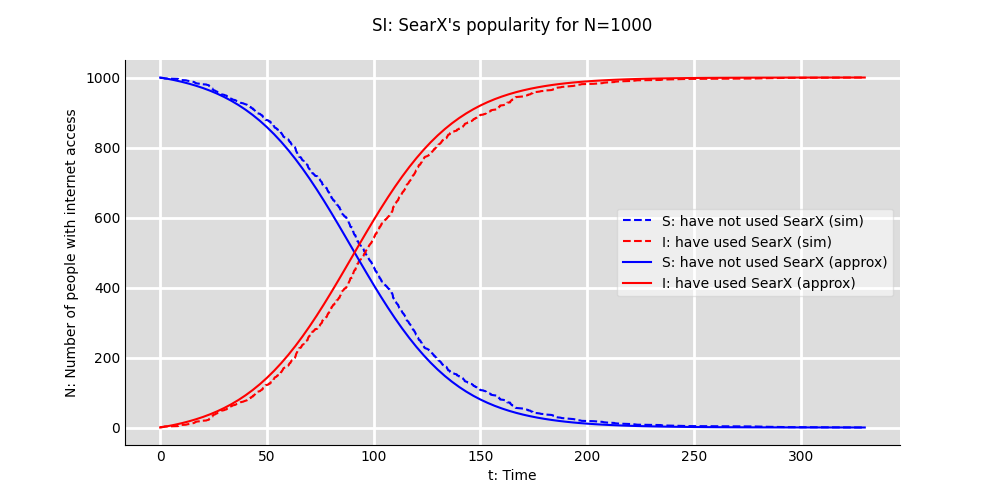
\includegraphics[width=0.8\linewidth]{si}
    \caption{Simulation‌ ‌of‌ ‌the‌ ‌SSA‌ ‌algorithm,‌ ‌applied‌ ‌to‌ ‌the‌ ‌SI‌ ‌model.‌‌}
    \label{fig:si}
\end{figure}

When‌‌ looking‌‌ at ‌‌the ‌‌simulation ‌‌results‌‌ from \autoref{fig:si}, ‌‌some‌‌ may‌‌ notice‌‌ a‌‌ change‌‌ in‌‌ the‌‌ values‌‌ of‌‌ the‌‌ axis,‌ $\Delta t$,‌‌ compared‌‌ to‌‌ the‌‌ previous‌‌ SI‌‌ model.‌‌ This‌‌ value‌‌ is‌‌ not‌‌ manually‌‌ configured,‌‌as‌‌ it‌‌ is‌‌ defined‌‌ based‌‌ on‌‌ the‌‌ time‌‌ instances‌‌ a‌‌ reaction‌‌ takes‌‌ place,‌‌during‌‌ runtime. ‌‌In‌‌ fact, $\Delta t$ ‌changes‌‌ each‌ ‌time‌ ‌the‌ ‌program‌ ‌is‌ ‌executed.‌ ‌The‌ ‌reason‌ ‌for‌ ‌this‌ ‌is‌ ‌because‌ ‌the‌ ‌Gillespie‌ ‌algorithm,‌‌ unlike‌ ‌most‌ ‌traditional‌ ‌ones,‌ ‌is not ‌interval-driven,‌ ‌but‌ ‌instead‌ ‌it‌ ‌is‌ ‌event-driven.

‌‌In‌ ‌the ‌‌interval-driven ‌‌methods,‌‌a‌‌ $\Delta t$‌ where‌‌ the‌‌ reaction ‌‌happens‌‌ is ‌‌manually ‌‌chosen.‌‌This‌‌ can‌‌ be‌ ‌inconvenient,‌ ‌since‌ ‌it‌ ‌requires‌ ‌trial-and-error‌ ‌to‌ ‌figure‌ ‌out‌ ‌a‌ $\Delta t$ ‌with‌ ‌reliable‌ ‌results.‌ ‌If‌ ‌the‌‌ propensities‌ ‌were‌ ‌to‌ ‌be‌ ‌changed,‌ ‌the‌ ‌$\Delta t$ ‌would‌ ‌have‌ ‌to‌ ‌be‌ ‌determined‌ ‌again‌ ‌by‌ ‌using‌ ‌brute‌‌ force‌ ‌in‌ ‌a‌ ‌non-automatic‌ ‌manner.‌ ‌Interval-driven‌ ‌methods‌ ‌can‌ ‌also‌ ‌be‌ ‌inefficient, since‌ ‌ many‌‌ random‌‌ intervals ‌‌would ‌‌have‌‌ to‌‌ be‌‌ generated‌‌ before‌‌ the‌‌ first‌‌ reaction‌‌ occurs,‌‌without ‌‌an ‌‌effect‌‌ on‌ ‌the‌ ‌system.‌‌

By‌ ‌contrast,‌ ‌the‌ ‌event-driven‌ ‌method‌ ‌consists‌ ‌of‌ ‌calculating‌ ‌the‌ ‌time‌ ‌until‌ ‌the‌ ‌next‌ ‌event‌‌ happens,‌ ‌then‌ ‌skipping‌ ‌time‌ ‌forward‌ ‌until‌ ‌that‌ ‌time‌ ‌is‌ ‌reached‌ ‌in‌ ‌order‌ ‌to‌ ‌execute‌ ‌the‌ ‌event.‌‌ This‌ ‌means‌ ‌that‌ ‌each‌ ‌iteration‌ ‌will‌ ‌respond‌ ‌to‌ ‌a ‌‌reaction ‌‌or ‌‌event,‌ meaning ‌‌that‌‌ iterations‌‌ will‌‌ not ‌‌be‌‌ wasted ‌‌in‌‌ time‌‌ instances‌‌ where‌‌ no‌‌ reaction‌‌ has‌‌ occurred,‌ which‌‌ typically ‌‌corresponds ‌‌to‌‌ the‌ ‌vast‌ ‌majority‌ ‌of‌ ‌time‌ ‌instances.‌ ‌This‌ ‌is‌ ‌a‌ ‌great‌ ‌advantage,‌ ‌in‌ ‌comparison‌ ‌to‌ ‌the‌‌ interval-driven‌ ‌method.‌

In‌ ‌the‌ ‌implemented‌ ‌code,‌ ‌based‌ ‌on‌ ‌an‌ ‌article‌ ‌written‌ ‌by‌‌ Andrew‌‌ Mellor [15‌], the‌‌ simulation‌‌ is‌‌ run‌ ‌over‌ ‌a‌ ‌randomly‌ ‌generated‌ ‌network,‌ ‌by‌ ‌using‌ ‌the‌ ‌networkx‌ ‌module.‌ ‌The‌ ‌module‌‌ SI Simulation,‌ ‌which‌ ‌takes‌ ‌responsibility‌ ‌for‌ ‌running‌ ‌the‌ ‌algorithm,‌ ‌takes‌ ‌in‌ ‌the‌ ‌following‌ ‌input:‌ ‌

A:‌ ‌Network‌ ‌where‌ ‌the‌ ‌simulation‌ ‌takes‌ ‌place.

$\lambda$:‌ ‌Contagion‌ ‌parameter,‌ ‌which‌ ‌represents‌ ‌the‌ ‌transition‌ ‌in‌ ‌the‌ ‌first‌ ‌reaction.

$\gamma$: ‌‌Spontaneous‌ ‌infection‌ ‌parameter,‌ ‌which‌ ‌represents‌ ‌the‌ ‌transition‌ ‌in‌ ‌the‌ ‌second‌ ‌reaction.‌

$I_0$: Initial‌ ‌infected‌ ‌fraction.‌ ‌

‌prop: Propensity‌‌ calculation ‌‌method.‌‌There‌‌ are ‌‌several ‌‌options‌‌ to ‌‌calculate‌‌ this‌‌ function,‌‌ but‌‌ by‌ ‌default‌ ‌it‌ ‌calculates‌ ‌all‌ ‌entries‌ ‌of‌ ‌the‌ ‌propensity‌ ‌function,‌ $\alpha_0$,‌ ‌at‌ ‌each‌ ‌iteration.

As‌ ‌for‌ ‌the‌ ‌actual‌ ‌Gillespie‌ ‌algorithm,‌ ‌it‌ ‌can‌ ‌be‌ ‌divided‌ ‌into‌ ‌the‌ ‌following‌ ‌steps:‌‌

\begin{enumerate} % TODO: add equations
    \item Generate‌ ‌two‌ ‌pseudo-random‌ ‌numbers,‌ $r_1$ and‌ ‌$r_2$,‌ ‌uniformly‌ ‌distributed‌ ‌in‌ ‌[0,‌ ‌1).
    \item Compute‌ ‌the‌ ‌propensity‌ ‌function‌ ‌$\alpha _i^m(t)$,‌ ‌for‌ ‌each‌ ‌node‌ ‌i‌ ‌and ‌‌reaction‌‌ m, ‌‌then‌‌ compute‌‌ the‌ ‌total‌ ‌propensity‌, $\alpha_0$.‌
    
        \begin{equation}
            \alpha_0 = \sum_\text{m=1}^M \sum_\text{i=1}^N \alpha_i^m(t)
        \end{equation}

    \item Compute‌ ‌the‌ ‌time‌ ‌until‌ ‌the‌ ‌next‌ ‌reaction‌ ‌takes‌ ‌place.‌
    
        \begin{equation} %TODO: change letter theta to τ
            \theta = \frac{1}{\alpha_0} * log(\frac{1}{r_1})
        \end{equation}

    \item Compute‌ ‌which‌ ‌reaction‌ ‌takes‌ ‌place‌ ‌at‌ ‌$t = t + weirdT$.‌ ‌In‌ ‌other‌‌ words,‌‌find ‌‌the ‌‌values ‌‌of ‌‌k‌‌ and‌ ‌j,‌ ‌where‌ ‌the‌ ‌following‌ ‌condition‌ ‌is‌ ‌satisfied:‌ ‌%TODO: add τ

        \begin{equation}
            \frac{1}{\alpha_0} \sum_\text{m=1}^\text{k-1} \sum_\text{i=1}^\text{j-1} \alpha_i^m(t) <= r_2 < \frac{1}{\alpha_0} \sum_\text{m=1}^k \sum_\text{i=1}^j \alpha_i^m(t) 
        \end{equation}

    \item Update‌ ‌the‌ ‌node‌ ‌states‌ ‌and‌ ‌propensities‌ ‌for‌ ‌the‌ ‌k-th‌ ‌reaction‌ ‌of‌ ‌the‌ ‌j-th‌ ‌node.‌ ‌
    \item Update‌ ‌propensities,‌ ‌by‌ ‌repeating‌ ‌the‌ ‌iteration,‌ ‌but‌ ‌for‌ ‌ ‌$t = t + weirdT$.‌
\end{enumerate}

A‌ ‌propensity‌ ‌function,‌ $\alpha_0$,‌ ‌which‌ ‌is‌ ‌computed‌ ‌in‌ ‌step‌ ‌2,‌ ‌describes‌ ‌the‌ ‌tendency‌ ‌of‌ ‌a‌ ‌reaction‌‌ occurring‌ ‌in‌ ‌the‌ ‌next‌ t ‌instance‌ ‌and‌ ‌is‌ ‌defined‌ ‌based‌ ‌on‌ ‌the‌ ‌value‌ ‌of‌ ‌the‌ ‌population‌ N [16‌].‌ 

\subsection{Applying‌ ‌the‌ ‌optimal‌ ‌control‌ ‌to‌ ‌the‌ ‌SI‌ ‌model}‌

Optimal‌ ‌control‌ ‌is‌ ‌a‌ ‌theory‌ ‌that‌‌ attempts‌‌ to‌‌ find‌‌ a‌‌ good,‌‌ usually‌‌ optimal,‌‌solution‌‌ in‌‌ a‌‌ dynamic‌‌ system.‌ ‌The‌ ‌system‌ ‌is‌ ‌described‌ ‌by‌ ‌an‌ ‌objective‌ ‌function‌ ‌ J ,‌ ‌and‌ ‌the‌‌ problem‌‌ often‌‌ is‌‌ to‌‌ find‌‌ values‌‌ that‌‌ minimize‌‌ or‌‌ maximize‌‌ this‌‌ function‌‌ over‌‌ an‌‌ interval‌‌ [17‌].‌‌ If‌‌ the‌‌ goal‌‌ is‌‌ to‌‌ maximize‌‌ J,‌‌ it‌ ‌is‌ ‌referred‌ ‌to‌ ‌as‌ ‌a‌ ‌value‌ ‌function.‌ ‌If‌ ‌the‌ ‌goal‌ ‌is‌ ‌to‌ ‌minimize‌ ‌ J ,‌ ‌it‌ ‌is‌ ‌referred‌ ‌to‌ ‌as‌ ‌a‌ ‌cost‌‌ function.‌ ‌In‌ ‌addition,‌ ‌restrictions‌ ‌are‌ ‌applied‌ ‌to‌ ‌the‌ ‌system.‌ ‌These‌ ‌restrictions‌ ‌consist‌ ‌of‌‌ equations‌ ‌that‌ ‌can‌ ‌be‌ ‌categorized‌ ‌into‌ ‌state‌ ‌restrictions‌ ‌and‌ ‌transition‌ ‌restrictions.

In‌ ‌the‌ ‌context‌ ‌of‌ ‌this‌ ‌work,‌ ‌it‌ ‌is‌ ‌intended‌ ‌to‌ ‌increase‌ ‌the‌ ‌popularity‌ ‌of‌ ‌SearX.‌ ‌There‌ ‌is‌ ‌more‌ ‌than‌‌ one‌ ‌way‌ ‌to‌ ‌formulate‌ ‌the‌ ‌model‌ ‌with‌ ‌this‌ ‌goal.‌‌ 

The‌ ‌simplest‌ ‌way‌ ‌to‌ ‌accomplish‌ ‌this‌ ‌goal‌ ‌is‌ ‌to‌ ‌introduce‌ ‌a‌ ‌control‌ ‌function,‌ ‌u(t),‌ ‌with‌ ‌a‌‌ descriptive‌ ‌meaning‌ ‌to‌ ‌be‌ ‌mentioned‌ ‌soon,‌ ‌that‌ ‌increases‌ ‌the‌ ‌number‌ ‌of‌ ‌people‌ ‌from‌ ‌the‌‌ Infectious‌ ‌group,‌ ‌that‌ ‌is,‌ ‌the‌ ‌number‌ ‌of‌ ‌people‌ ‌who‌ ‌have‌ ‌used‌ ‌SearX.‌ ‌Since‌ ‌it‌ ‌is‌‌ intended‌‌ to‌‌ maximize‌ J ,‌ ‌this‌ ‌objective‌ ‌function‌ ‌will‌ ‌be‌ ‌a‌ ‌value‌ ‌function‌ ‌defined‌ ‌by‌ ‌the‌ ‌following‌ ‌equation:‌ 

\begin{equation}
    \text{max J(t)} = \int_\text{$t_i=2014$}^\text{$t_f=2050$} [ I(t) + u^2(t) ] dt
\end{equation}

The‌ ‌ODEs‌ ‌of‌ ‌the‌ ‌SI‌ ‌model‌ ‌will‌ ‌also‌ ‌need‌ ‌a‌ ‌few‌ ‌adjustments,‌ ‌as‌ ‌presented‌ ‌below:‌‌

% TODO: add equations 

It‌‌ was‌‌ also‌‌ decided‌‌ to‌‌ apply‌‌ a‌‌ restriction‌‌ to‌‌ the‌‌ optimal‌‌ control‌‌ function,‌‌ u(t). ‌‌That‌‌ restriction‌‌ is $0 \le u(t) \le umax < 1$‌‌,‌ ‌where‌ $umax=0.5$.‌ ‌In‌ ‌the‌ ‌context‌ ‌of‌ ‌SearX,‌ ‌u(t) ‌represents‌ ‌a‌ ‌strong‌‌ advertisement‌‌ campaign‌‌ that‌‌ helps‌‌ convincing‌‌ people‌‌ who‌‌ have not ever‌‌ used‌‌ the‌‌ engine‌‌ to‌‌ use‌‌ it ‌‌Mathematically‌‌ speaking,‌‌ u(t) ‌increases‌‌ the‌‌ speed‌‌ at‌‌ which‌‌ I(t) ‌increases.‌‌ It‌‌ is‌‌ important‌‌ to‌‌ mention‌ ‌that‌ ‌the‌ ‌value‌ ‌of‌ u ‌cannot‌‌ reach‌‌ the‌‌ same‌‌ value‌‌ as‌‌ $u_max$,‌‌ because‌‌ an‌‌ advertisement‌‌ campaign‌ ‌never‌ ‌reaches‌ ‌exactly‌ ‌100\% ‌of‌ ‌the‌ ‌individuals‌ ‌from‌ ‌the‌ ‌ S(t) ‌group.‌‌

By‌ ‌simulating‌ ‌the‌ ‌SI‌ ‌with‌ ‌this‌ ‌particular‌ ‌optimal‌ ‌control,‌ ‌the‌ ‌results‌ ‌from‌ \autoref{fig:plts1_SI_optimal_control_I}‌ ‌are‌ ‌obtained.‌ ‌

\begin{figure}[h]
    \centering
    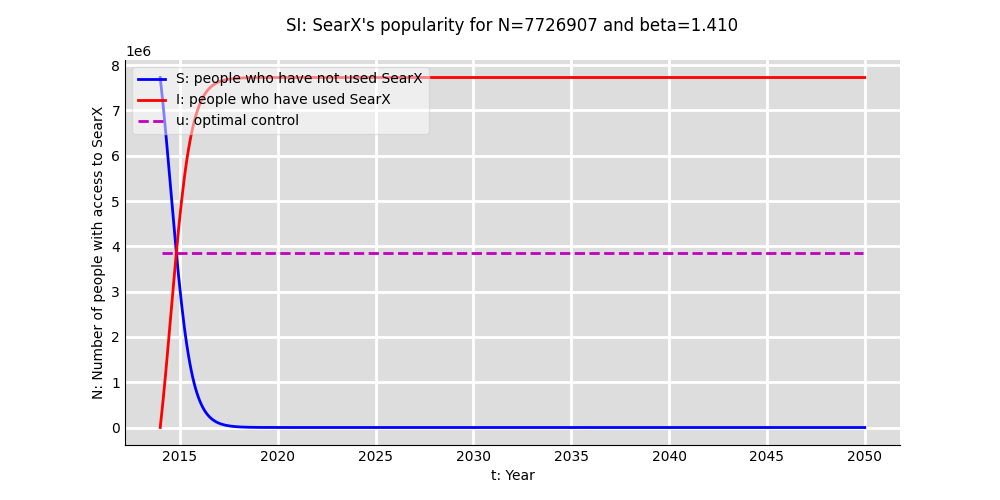
\includegraphics[width=0.8\linewidth]{plts1_SI_optimal_control_I}
    \caption{‌Simulation‌ ‌with‌ ‌optimal‌ ‌control‌ ‌applied‌ ‌to‌ ‌ I(t) ,‌ ‌in‌ ‌the‌ ‌SI‌ ‌model.‌‌‌}
    \label{fig:plts1_SI_optimal_control_I}
\end{figure}

It‌ ‌is‌ ‌interesting‌ ‌to‌ ‌notice‌ ‌how‌ ‌ u(t) ‌is‌ ‌constant‌ ‌through‌ ‌time.‌ ‌The‌ ‌reason‌ ‌for‌ ‌this‌ ‌might‌ ‌be‌‌ because,‌ ‌in‌ ‌the‌ ‌ S'(t) ‌function,‌ ‌ u(t) × S ‌is‌ ‌incremented,‌ ‌while‌ ‌in‌ ‌the‌ ‌ I'(t) ‌function,‌ ‌the‌ ‌same‌‌ value,‌ u(t) × S ,‌ ‌is‌ ‌decremented.‌

An‌ ‌important‌ ‌conclusion‌ ‌to‌ ‌take‌ ‌from‌ ‌this‌ ‌simulation‌ ‌\autoref{fig:plts1_SI_optimal_control_I}‌ ‌is‌ ‌that,‌ ‌compared‌ ‌to‌ ‌the‌‌ simulations‌ ‌from‌ ‌[5],‌ ‌the‌ ‌increase‌ ‌of‌ ‌the‌ ‌ I(t) ‌is‌ ‌faster‌ ‌as‌ ‌well‌ ‌as‌ ‌the‌ ‌decrease‌ ‌of‌ ‌ S(t).‌

A‌ ‌similar‌ ‌but‌ ‌different‌‌ approach‌‌ can‌‌ be‌‌ made‌‌ when‌‌ it‌‌ comes‌‌ to‌‌ applying‌‌ the‌‌ optimal‌‌ control‌‌ to‌‌ the‌ ‌SI‌ ‌model,‌ ‌including‌ ‌in‌ ‌the‌ ‌context‌ ‌of‌ ‌SearX.‌ ‌The‌ ‌value‌ ‌function‌ ‌ J(t),‌ ‌restriction‌ ‌and‌‌ descriptive‌‌ meaning‌‌ of‌‌ u(t),‌‌which‌‌ have‌‌ been‌‌ previously‌‌ mentioned,‌‌ stay‌‌ unchanged.‌‌ However,‌‌ instead‌ ‌of‌ ‌only‌ ‌increasing‌ ‌the‌ ‌value‌ ‌of‌ ‌ I(t) ‌directly,‌ ‌the‌ "transmission" ‌value‌ ‌can‌ ‌also‌ ‌be‌‌ increased,‌ ‌as‌ ‌presented‌ ‌in‌ ‌the‌ ‌updated‌ ‌ODEs:‌

% TODO: add equations

With‌ ‌this‌ ‌particular‌ ‌optimal‌ ‌control,‌ ‌the‌ ‌respective‌ ‌simulation‌ ‌is‌ ‌presented‌ ‌in‌ \autoref{fig:plts1_SI_optimal_control_I}.

\begin{figure}[h]
    \centering
    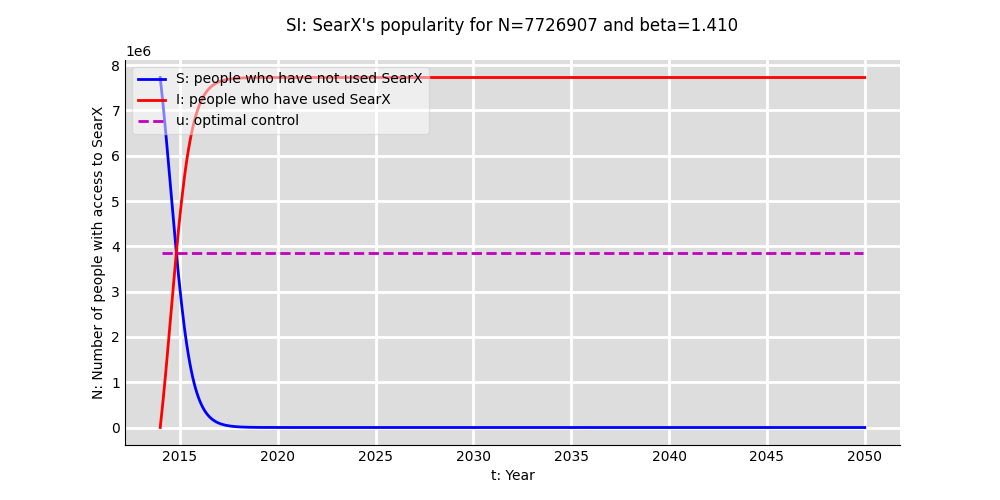
\includegraphics[width=0.8\linewidth]{plts1_SI_optimal_control_I}
    \caption{‌‌Simulation‌ ‌with‌ ‌optimal‌ ‌control‌ ‌applied‌ ‌to‌ ‌the‌ ‌"transmission"‌ ‌value,‌ ‌in‌ ‌the‌ ‌SI‌ ‌model.‌‌‌}
    \label{fig:plts1_SI_optimal_control_transmition}
\end{figure}

It‌ ‌is‌ ‌expected‌ ‌that‌ ‌the‌ ‌simulations‌ ‌from‌ \autoref{fig:plts1_SI_optimal_control_I}‌ ‌and‌ ‌9\autoref{fig:plts1_SI_optimal_control_transmition} ‌are‌ ‌exactly‌ ‌the‌ ‌same.‌ ‌The‌ ‌ODEs‌‌
developed‌‌ for‌‌ these‌‌ simulations,‌‌despite‌‌ being‌‌ different,‌‌express‌‌ the‌‌ same‌‌ solution.

Both‌ ‌simulations,‌ presented‌ ‌in‌ \autoref{fig:plts1_SI_optimal_control_I}‌ ‌and‌ ‌9\autoref{fig:plts1_SI_optimal_control_transmition},‌ ‌were‌ ‌created‌ ‌by‌ ‌using‌ ‌the‌ ‌AMPL‌  (A‌‌ Mathematical‌ ‌Programming‌ ‌Language)‌ ‌and‌ ‌python‌ ‌programming‌ ‌languages.‌ ‌The‌ ‌AMPL‌ ‌code‌‌ was‌ ‌executed‌ ‌in‌ ‌the‌ ‌NEOS‌  (Network-Enabled‌ ‌Optimization‌ ‌System)‌ ‌server‌ ‌[18].‌ ‌The‌ ‌AMPL‌‌ code‌ ‌was‌ ‌based‌ ‌on‌ ‌an‌ ‌unpublished‌ ‌report‌ ‌done‌ ‌by‌ ‌a‌ ‌computational‌ ‌engineering‌ ‌student‌ ‌at‌‌ University‌ ‌of‌ ‌Aveiro‌ ‌[19].‌

\subsection{Beyond the SI model}

The‌ ‌SI‌ ‌model,‌ ‌perhaps‌ ‌due‌ ‌to‌ ‌its‌ ‌simplicity,‌ ‌is‌ ‌one‌ ‌of‌ ‌the‌ ‌most‌ ‌naive‌ ‌models‌ ‌among‌ ‌the‌‌ compartmental‌ ‌models‌ ‌that‌ ‌originated‌ ‌from‌ ‌epidemiology‌ [20].‌ ‌For‌ ‌instance,‌ ‌in‌ ‌the‌ ‌context‌ ‌of‌‌ SearX ‌‌the‌‌ SI‌‌ model‌‌ is‌‌ not‌‌ capable‌‌ of‌‌ presenting‌‌ the‌‌ number‌‌ of‌‌ people‌‌ who‌‌ are‌‌ currently‌‌ using‌‌ SearX ‌‌To‌‌ forecast‌‌ the‌‌ popularity‌‌ of‌‌ SearX ‌‌it‌‌ is‌‌ usually‌‌ more‌‌ relevant‌‌ to‌‌ determine‌‌ the‌‌ number‌‌ of‌ ‌current‌ ‌users‌ ‌than‌ ‌the‌ ‌number‌ ‌of‌ ‌people‌ ‌who‌ ‌have‌ ‌used‌ ‌the‌ ‌engine. ‌‌Afterall,‌‌ just‌‌ because‌‌ many‌ ‌people‌ ‌have‌ ‌used‌ ‌SearX,‌ ‌it‌ does not ‌mean‌ ‌that‌ ‌all‌ ‌of‌ ‌them‌ ‌are‌ ‌currently‌ ‌using‌ ‌the‌ ‌engine.‌‌

How‌ ‌exactly‌ ‌can‌ ‌the‌ ‌number‌ ‌of‌ ‌current‌ ‌users‌ ‌of‌ ‌SearX‌ ‌be‌ ‌tracked? ‌A‌ ‌software‌ ‌mechanism‌‌ would‌ ‌be‌ ‌required‌ ‌for‌ ‌this.‌ ‌For‌ ‌example,‌ ‌it‌ ‌can‌ ‌be‌ ‌supposed‌ ‌that‌ ‌the‌ ‌software‌ ‌allows‌ ‌the‌‌ operations‌‌ of‌‌ creating‌‌ and‌‌ deleting‌‌ an‌‌ user‌‌ account‌‌ since‌‌ the‌‌ first‌‌ day‌‌ it‌‌ was‌‌ launched.‌‌ In‌‌ other‌‌ words,‌ ‌whenever‌ ‌current‌ ‌users‌ ‌are‌ ‌being‌ ‌mentioned,‌ ‌it‌ ‌means‌ ‌the‌ ‌number‌ ‌of‌ ‌active‌ ‌user‌‌ accounts‌ ‌in‌ ‌SearX.‌

\subsubsection{SIR‌ ‌model‌}

A‌‌ solution‌‌ for‌‌ this‌‌ issue‌‌ is‌‌ to‌‌ add‌‌ a‌‌ new‌‌ state,‌‌ expressed‌‌ by‌‌ R(t), ‌‌that‌‌ represents‌‌ the‌‌ Recovered‌‌ (R) ‌group.‌ ‌This‌ ‌implies‌ ‌changes‌ ‌in‌ ‌the‌ ‌descriptive‌ ‌meaning‌ ‌of‌ ‌the‌ ‌functions,‌ ‌as‌ ‌shown‌ ‌in‌ ‌table‌ ‌2.

\begin{tabularx}{1\textwidth} { 
    | >{\centering\arraybackslash}X 
    || >{\centering\arraybackslash}X | }
   \hline
   S(t) & Number‌ ‌of‌ ‌people‌ ‌who‌ ‌have‌ ‌never‌ ‌been‌ ‌SearX‌ ‌users‌ ‌at‌ ‌time‌ ‌t.‌ ‌\\
   \hline
   I(t)  & Number‌ ‌of‌ ‌people‌ ‌who‌ ‌are‌ ‌SearX‌ ‌users‌ ‌at‌ ‌time‌ ‌t.‌ \\
   \hline
   R(t)  & Number‌ ‌of‌ ‌people‌ ‌who‌ ‌are‌ ‌no‌ ‌longer‌ ‌SearX‌ ‌users‌ ‌at‌ ‌time‌ ‌t.‌ \\
  \hline
\end{tabularx}

By‌ ‌convention,‌ ‌the‌ ‌initial‌ ‌conditions‌ ‌are:‌ ‌

%TODO: add equations

As‌ ‌for‌ ‌the‌ ‌actual‌ ‌model,‌ ‌the‌ ‌model‌ ‌can‌ ‌be‌ ‌expressed‌ ‌by‌ ‌the‌ ‌diagram‌ ‌presented‌ ‌by‌ \autoref{fig:SIR}.

\begin{figure}[h]
    \centering
    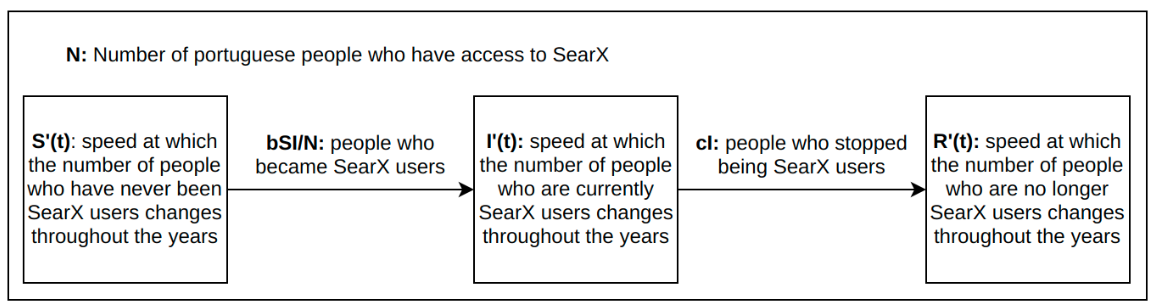
\includegraphics[width=0.7\linewidth]{SIR}
    \caption{‌‌Simulation‌ ‌with‌ ‌optimal‌ ‌control‌ ‌applied‌ ‌to‌ ‌the‌ ‌"transmission"‌ ‌value,‌ ‌in‌ ‌the‌ ‌SI‌ ‌model.‌‌‌}
    \label{fig:SIR}
\end{figure}

The‌ ‌model‌ ‌can‌ ‌also‌ ‌be‌ ‌formulated‌ ‌by‌ ‌the‌ ‌following‌ ‌ODEs‌:‌

%TODO: add equations

In‌‌ this‌‌ model,‌‌it‌‌ is‌‌ being‌‌ assumed‌‌ that‌‌ those‌‌ who‌‌ no‌‌ longer‌‌ use‌‌ the‌‌ engine‌‌ cannot‌‌ influence‌‌ the‌‌ current‌ ‌users‌ ‌to‌ ‌abandon‌ ‌the‌ ‌service,‌ ‌hence‌ ‌the‌ ‌expression‌ ‌ c I ,‌ ‌where‌ ‌c,‌ ‌known‌ ‌as‌‌ recovery‌‌ rate,‌ ‌represents‌ ‌the‌ ‌rate‌ ‌at‌ ‌which‌ ‌people‌ ‌stop‌ ‌being‌ ‌users‌ ‌of‌ ‌the‌ ‌engine.‌ ‌This‌ ‌expression‌ ‌is‌‌ decremented‌ ‌in‌ ‌I'(t)‌‌and‌ ‌decremented‌ ‌in‌ ‌R'(t),‌ ‌because‌ ‌the‌ ‌people‌ ‌who‌ ‌abandon‌ ‌the‌ ‌service‌‌ transition‌ ‌from‌ ‌the‌ ‌Infectious‌ ‌group‌ ‌to‌ ‌the‌ ‌Recovered‌ ‌group.‌‌

To‌‌ improve ‌‌the ‌‌popularity ‌‌of‌‌ SearX,‌‌it ‌‌is ‌‌evident‌‌ that‌‌ the‌‌ number‌‌ of‌‌ current‌‌ users‌‌ of‌‌ the‌‌ engine‌‌ needs‌ ‌to‌ ‌increase.‌ ‌This‌ ‌is‌ ‌accomplished‌ ‌by‌ ‌increasing‌ ‌I'(t)‌ ‌and‌ ‌decreasing‌ ‌S'(t)‌ ‌and‌ ‌R'(t),‌ ‌by‌‌
increasing‌ ‌b‌ ‌and‌ ‌decreasing‌ ‌c.‌

The‌ ‌results‌ ‌of‌ ‌the‌ ‌simulation‌ ‌are‌ ‌presented‌ ‌in‌ \autoref{fig:si}.‌‌

\begin{figure}[h]
    \centering
    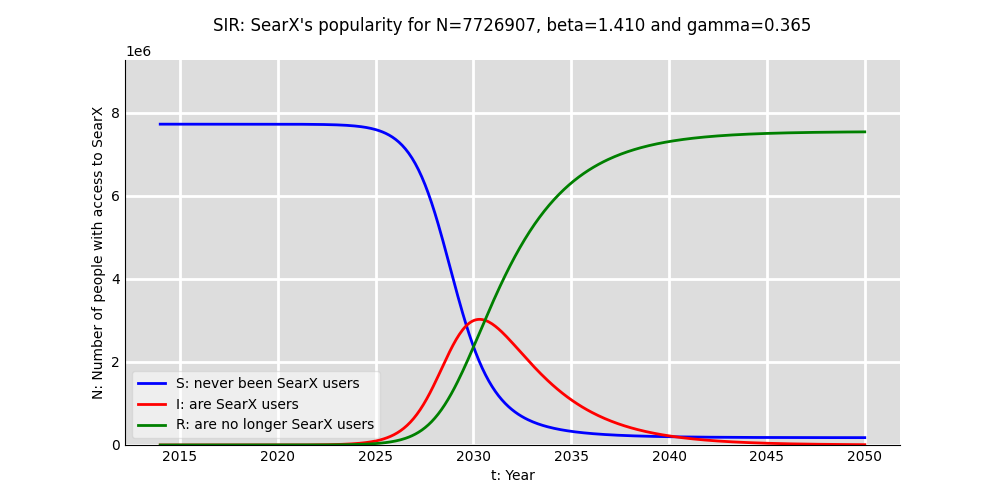
\includegraphics[width=0.8\linewidth]{plts3_SIR2}
    \caption{‌‌Simulation‌ ‌of‌ ‌the‌ ‌SIR‌ ‌model,‌ ‌adapted‌ ‌to‌ ‌the‌ ‌context‌ ‌of‌ ‌SearX.‌‌‌‌}
    \label{fig:plts3_SIR}
\end{figure}

\subsubsection{SIRI model}

An‌‌ issue‌‌ of‌‌ the‌‌ SIR‌‌ model‌‌ previously‌‌ developed‌‌ is‌‌ that,‌‌ once‌‌ people‌‌ stop‌‌ using‌‌ the‌‌ engine,‌‌ they‌‌ cannot‌‌ become‌‌ a‌‌ SearX‌‌ user‌‌ again.‌‌ To‌‌ fix‌‌ this,‌‌no‌‌ new‌‌ state‌‌ needs‌‌ to‌‌ be‌‌ added,‌‌ therefore‌‌ the‌‌ descriptive‌ ‌meaning‌ ‌of‌ ‌those‌ ‌states‌ ‌will‌ ‌stay‌ ‌the‌ ‌same. ‌‌Consequently,‌‌ the‌‌ initial‌‌ conditions‌‌ do‌‌ not‌‌ have‌‌ to‌‌ be‌‌ updated ‌‌and‌‌ therefore‌‌ will‌‌ stay‌‌ unchanged.‌‌ However,‌‌ a‌‌ new‌‌ transition‌‌ needs‌‌ to‌‌ be‌‌added ‌‌so‌‌ the‌‌ model‌‌ diagram‌‌ will‌‌ have‌‌ to‌‌ be‌‌ updated‌‌ to‌‌ the‌‌ following,‌‌ as‌‌ presented‌‌ in‌‌ \autoref{fig:plts3_SIR}:‌

\begin{figure}[h]
    \centering
    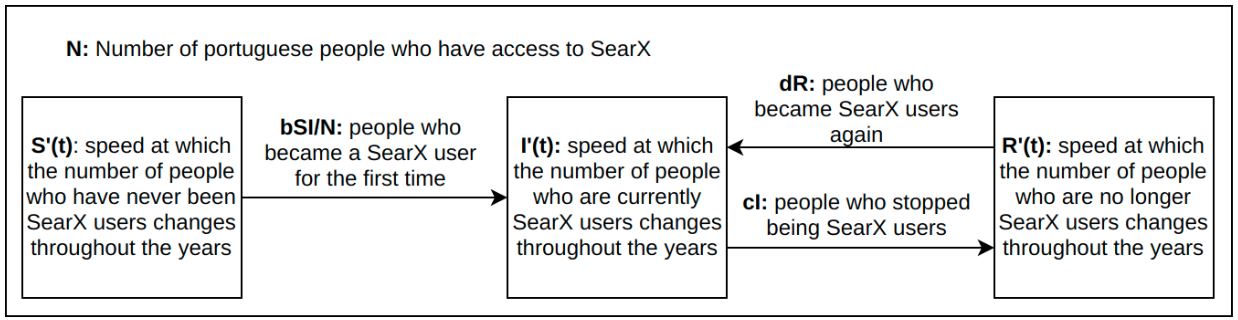
\includegraphics[width=0.8\linewidth]{SIRI}
    \caption{‌SIRI‌ ‌model‌ ‌diagram,‌ ‌applied‌ ‌to‌ ‌the‌ ‌context‌ ‌of‌ ‌SearX.‌}
    \label{fig:SIRI}
\end{figure}

This‌ ‌model‌ ‌is‌ ‌expressed‌ ‌by‌ ‌the‌ ‌following‌ ‌ODEs:‌

\begin{equation}
    \begin{subequations}
        % TODO: add new line between equations
        \frac{dS}{dt} = - \frac{bSI}{N}
        \frac{dI}{dt} = \frac{bSI}{N} - cI + dR
        \frac{dR}{dt} = cI - dR
    \end{subequations}
    \label{eq:SEIRIinitialConditions}
\end{equation}

The‌ ‌parameter‌ ‌d‌ ‌represents‌ ‌the‌ ‌retransmission‌ ‌ratio,‌ ‌that‌ ‌is,‌ ‌the‌ ‌ratio‌ ‌of ‌‌people‌‌ who‌‌ become‌‌ SearX‌ ‌users‌ ‌again.‌ ‌For‌ ‌simplification,‌‌it ‌‌was ‌‌decided ‌‌that‌‌ people‌‌ who‌‌ are‌‌ SearX‌‌ users‌‌ cannot‌‌ influence‌ ‌those‌ ‌who‌ ‌are‌ ‌not‌ ‌SearX‌ ‌users,‌ ‌but‌ ‌have‌ ‌been‌ ‌in‌ ‌the‌ ‌past,‌ ‌into‌ ‌using‌ ‌the‌ ‌engine‌‌ again,‌ ‌hence‌ ‌the‌ ‌expression‌ ‌dR.‌ ‌This‌ ‌expression‌ ‌is‌ ‌incremented‌ ‌in‌ ‌I'(t)‌ ‌and‌ ‌decremented‌ ‌in‌‌ R'(t),‌ ‌because‌ ‌when‌ ‌people‌ ‌become‌ ‌SearX‌ ‌users‌ ‌again,‌ ‌those‌ ‌people‌ ‌transition‌ ‌from‌ ‌the‌‌ Recovered‌ ‌group‌ ‌to‌ ‌the‌ ‌Infectious‌ ‌group.‌ ‌

To‌ ‌improve‌ ‌the‌ ‌popularity‌ ‌of‌ ‌SearX,‌ ‌it‌ ‌is‌ ‌necessary‌ ‌for‌ ‌the‌ ‌number‌ ‌of‌ ‌current‌ ‌SearX‌ ‌users‌‌ to‌‌ increase. ‌‌This‌‌ is‌‌ accomplished‌‌ by‌‌ increasing ‌‌I’(t) ‌‌and‌‌ decreasing‌‌ S'(t)‌‌ and‌‌ R'(t),‌‌ by‌‌ increasing‌‌ b‌‌ and‌ ‌d‌ ‌and‌ ‌decreasing‌ ‌c.‌

The‌ ‌results‌ ‌of‌ ‌the‌ ‌simulation‌ ‌of‌ ‌this‌ ‌model‌ ‌are‌ ‌presented‌ ‌in‌ \autoref{fig:plts4_SIRI2}.

\begin{figure}[h]
    \centering
    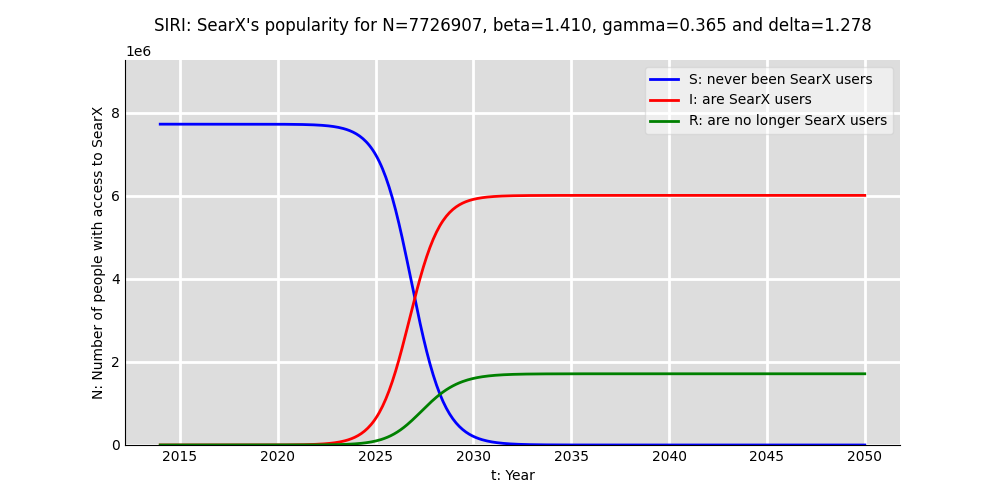
\includegraphics[width=0.8\linewidth]{plts4_SIRI2}
    \caption{‌‌Simulation‌ ‌of‌ ‌the‌ ‌SIR‌I ‌model,‌ ‌adapted‌ ‌to‌ ‌the‌ ‌context‌ ‌of‌ ‌SearX.‌‌‌‌}
    \label{fig:plts4_SIRI2}
\end{figure}

\subsubsection{SEIRI model}

To ‌‌develop‌‌ a‌‌ more‌‌ accurate‌‌ model,‌‌ a‌‌ distinction‌‌ can‌‌ be‌‌ made‌‌ between‌‌ those‌‌ who‌‌ are‌‌ unfamiliar‌‌ with‌‌ SearX‌‌ and‌‌ have‌‌ never‌‌ been‌‌ users‌‌ of‌‌ the‌‌ engine ‌‌and‌‌ those‌‌ who‌‌ have‌‌ never‌‌ been‌‌ users‌‌ of‌‌ the‌ ‌engine‌ ‌despite‌ ‌their‌ ‌familiarity‌ ‌with‌ ‌the‌ ‌software.‌ ‌In‌ ‌order‌ ‌to‌ ‌make‌ ‌this‌‌ distinction,‌‌ a‌‌ new‌‌ state‌ ‌needs‌ ‌to‌ ‌be‌ ‌added.‌ ‌This‌ ‌requires‌ ‌an‌ ‌update‌ ‌in‌ ‌the‌ ‌descriptive‌ ‌meaning‌ ‌of‌ ‌the‌ ‌required‌‌
functions,‌ ‌presented‌ ‌in‌ ‌table‌ ‌3.‌

\begin{tabularx}{1\textwidth} { 
    | >{\centering\arraybackslash}X 
    || >{\centering\arraybackslash}X | }
   \hline
   S(t) & Number‌ ‌of‌ ‌people‌ ‌who‌ ‌have‌ ‌never‌ ‌been‌ ‌SearX‌ ‌users‌ ‌and‌ ‌are‌ ‌not‌ ‌familiar‌ ‌with‌‌ the‌ ‌engine,‌ ‌at‌ ‌time‌ ‌t.‌ ‌‌ ‌\\
   \hline
   E(t) & Number‌ ‌of‌ ‌people‌ ‌who‌ ‌have‌ ‌never‌ ‌been‌ ‌SearX‌ ‌users‌ ‌but‌ ‌are‌ ‌familiar‌ ‌with‌ ‌the‌‌ engine,‌ ‌at‌ ‌time‌ ‌t.‌ ‌\\
   \hline
   I(t)  & Number‌ ‌of‌ ‌people‌ ‌who‌ ‌are‌ ‌SearX‌ ‌users‌ ‌at‌ ‌time‌ ‌t.‌ ‌‌ \\
   \hline
   R(t)  & Number‌ ‌of‌ ‌people‌ ‌who‌ ‌are‌ ‌no‌ ‌longer‌ ‌SearX‌ ‌users‌ ‌at‌ ‌time‌ ‌t.‌ ‌‌ \\
  \hline
\end{tabularx}

By‌ ‌convention,‌ ‌the‌ ‌initial‌ ‌conditions‌ ‌are:‌‌

\begin{equation}
    \begin{subequations}
        % TODO: add new line between equations
        % TODO: fix S(2014) = N − E(2014) − I(2014) − R(2014) = 7726907 − 0 − 1 − 0 = 7726906
        E(2014) = 0
        I(2014) = 1
        R(2014) = 0
        \frac{dR}{dt} = cI - dR
    \end{subequations}
    \label{eq:SEIRIinitialConditions}
\end{equation}

The‌ ‌SEIR‌ ‌model‌ ‌itself‌ ‌can‌ ‌be‌ ‌presented‌ ‌by‌ ‌the‌ ‌following‌ ‌diagram‌ ‌presented‌ ‌in‌ \autoref{fig:SEIRI}.‌

\begin{figure}[h]
    \centering
    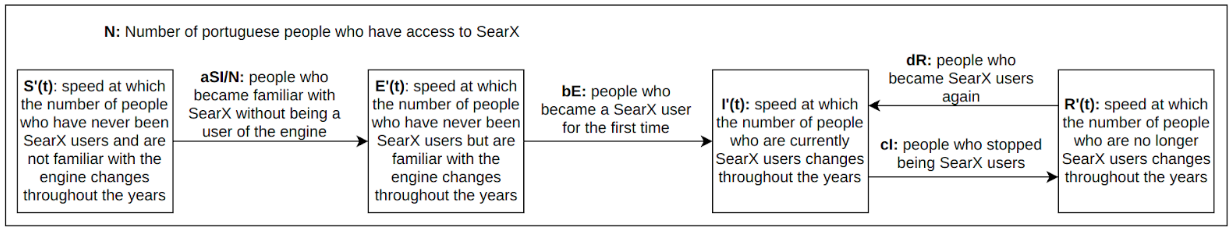
\includegraphics[width=1\linewidth]{SEIRI}
    \caption{SEIRI‌ ‌model‌ ‌diagram,‌ ‌applied‌ ‌to‌ ‌the‌ ‌context‌ ‌of‌ ‌SearX.‌}
    \label{fig:SEIRI}
\end{figure}

This‌ ‌model‌ ‌can‌ ‌be‌ ‌formally‌ ‌expressed‌ ‌by‌ ‌the‌ ‌following‌ ‌ODEs:‌

\begin{equation}
    \begin{subequations}
        % TODO: add new line between equations
        \frac{dS}{dt} = - \frac{aSI}{N} 
        \frac{dE}{dt} = \frac{aSI}{N} - bE 
        \frac{dI}{dt} = bE - cI + dR 
        \frac{dR}{dt} = cI - dR
    \end{subequations}
    \label{eq:SEIRIode}
\end{equation}

This‌ ‌model‌ ‌assumes‌ ‌that‌ ‌the‌ ‌SearX‌ ‌users‌ ‌can‌ ‌only‌ ‌influence‌ ‌someone‌ ‌from‌ ‌the‌ ‌Susceptible‌‌ group‌ ‌to‌ ‌be‌ ‌familiar‌ ‌with‌ ‌the‌ ‌engine,‌ ‌that‌ ‌is,‌ ‌transition‌ ‌to‌ ‌the‌ ‌Exposed‌ ‌(E)‌ ‌group.‌ ‌Roughly‌‌ speaking, ‌‌this‌‌ decision‌‌ was‌‌ based‌‌ on‌‌ the‌‌ popular‌‌ saying‌‌ "you‌‌ can‌‌ take‌‌ a‌‌ horse‌‌ to‌‌ the‌‌ water‌‌ but‌‌ you‌ ‌cannot‌ ‌make‌ ‌it‌ ‌drink".‌

The‌ ‌results‌ ‌of‌ ‌the‌ ‌simulation‌ ‌of‌ ‌this‌ ‌model‌ ‌are‌ ‌presented‌ ‌in‌ \autoref{fig:plts6_SEIRI2}.‌

\begin{figure}[h]
    \centering
    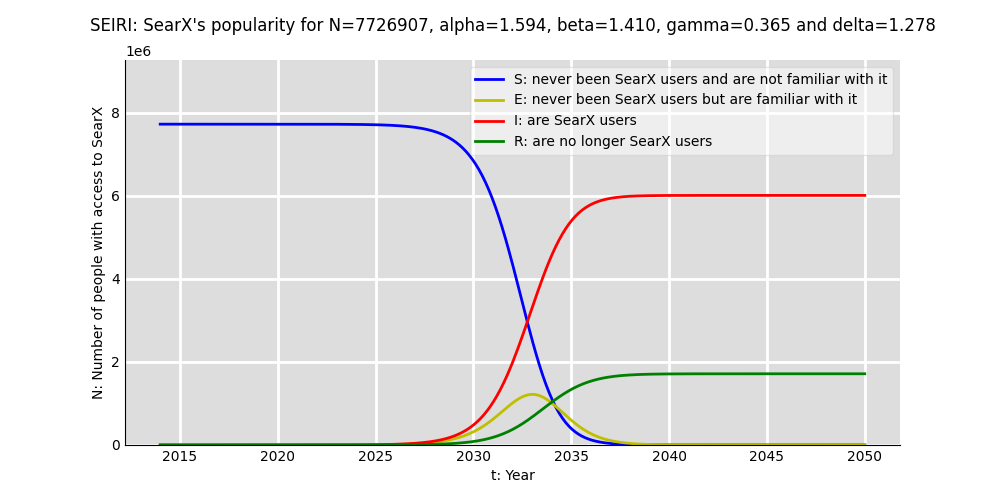
\includegraphics[width=0.8\linewidth]{plts6_SEIRI2}
    \caption{‌‌‌ ‌Simulation‌ ‌of‌ ‌the‌ ‌SEIR‌I ‌model,‌ ‌adapted‌ ‌to‌ ‌the‌ ‌context‌ ‌of ‌SearX.‌‌‌‌‌‌‌}
    \label{fig:plts6_SEIRI2}
\end{figure}

\section{Churn}

There ‌‌are‌‌ several‌‌ ways‌‌ to‌‌ model‌‌ and‌‌ simulate‌‌ the‌‌ popularity‌‌ of‌‌ SearX,‌‌but‌‌ how‌‌ exactly‌‌ can‌‌ the‌‌ popularity‌ ‌of‌ ‌an‌ ‌engine‌ ‌be‌ ‌increased?‌

For‌ ‌those‌ ‌who‌ ‌are‌ ‌familiar‌ ‌with‌ ‌the‌ ‌notion‌ ‌of‌ ‌optimal‌ ‌control,‌ ‌a‌ ‌descriptive‌ ‌meaning‌ ‌could‌‌ be‌‌ given‌ ‌to‌ ‌an‌ ‌optimal‌ ‌control‌ ‌function,‌ ‌such‌ ‌as‌ ‌an‌ ‌advertisement‌ ‌campaign.‌ ‌Then,‌‌that‌‌ function‌‌ could‌ ‌be‌ ‌integrated‌ ‌into‌ ‌a‌ ‌SI‌ ‌model,‌ ‌which‌ ‌has‌ ‌been‌ ‌done‌ ‌in‌ ‌a‌ ‌previous‌ ‌section,‌ ‌or‌ ‌into‌ ‌any‌‌ other‌ ‌model‌ ‌that‌ ‌has‌ ‌been‌ ‌developed‌ ‌throughout‌ ‌this‌ ‌report.‌‌

For‌‌ those ‌‌who‌‌ are‌‌ not ‌‌familiar ‌‌with‌‌ the‌‌ concept‌‌ of‌‌ optimal‌‌ control,‌‌ however,‌‌the‌‌ first ‌‌thought‌‌ that‌‌ comes‌‌ into ‌‌mind‌‌ when‌‌ thinking ‌‌about ‌‌strategies ‌‌to ‌‌improve‌‌ the ‌‌popularity‌‌ of‌‌ a‌‌ software ‌‌product‌‌ or‌ ‌service‌ ‌is‌ ‌to‌ ‌increase‌ ‌the‌ ‌number‌ ‌of‌ ‌new‌ ‌users.‌ ‌Nonetheless,‌ ‌if‌ ‌the‌ ‌number‌ ‌of‌ ‌users‌‌ abandoning‌ ‌the‌ ‌product‌ ‌is‌ ‌not‌ ‌taken‌ ‌into‌ ‌consideration,‌ ‌the‌ ‌measurement‌ ‌of‌ ‌the ‌‌popularity‌‌ of‌‌ that‌ ‌technology‌ ‌will‌ ‌not‌ ‌be‌ ‌as‌ ‌accurate, if‌ ‌not‌ ‌accurate‌ ‌at‌ ‌all.‌‌

For‌ ‌example,‌ ‌assuming‌ ‌that‌ ‌the‌ ‌intent‌ ‌of‌ ‌SearX‌ ‌is‌ ‌to ‌‌increase‌‌ its‌‌ popularity,‌‌ is‌‌ it‌‌ preferable‌‌ to‌‌ have‌‌ five‌‌ hundred‌‌ new‌‌ users‌‌ in‌‌ the‌‌ first‌‌ month‌‌ SearX‌‌ was‌‌ launched,‌‌or‌‌ five‌‌ million‌‌ new‌‌ users‌‌ in‌‌ that‌ ‌month?‌ ‌When‌ ‌answering‌ ‌this‌‌ question, ‌‌the‌‌ first‌‌ instinct‌‌ might‌‌ be‌‌ to‌‌ assume‌‌ that‌‌ the‌‌ latter‌‌ option‌ ‌is‌ ‌the‌ ‌correct‌ ‌answer.‌ ‌However,‌ ‌that‌ ‌would‌ ‌be‌ ‌a‌ ‌naive‌ ‌response,‌ ‌since‌ ‌it‌ ‌can‌ ‌be‌‌ preferable‌‌ to‌‌ have‌‌ 5‌‌ hundred‌‌ new‌‌ users‌‌ per‌‌ month‌‌ over‌‌ five‌‌ millions.‌‌ For‌‌ instance,‌‌ gaining‌‌ five‌‌ hundred‌ ‌users‌ ‌and‌ ‌losing‌ ‌one‌ ‌hundred‌ ‌users‌ ‌in‌ ‌the‌ ‌first‌ ‌month‌ ‌the‌ ‌engine‌ ‌was‌ ‌launched‌ ‌is‌‌ better‌‌ than‌‌ gaining‌‌ 5‌‌ million‌‌ users‌‌ and‌‌ losing‌‌ all‌‌ of‌‌ them,‌‌ with‌‌ the‌‌ exception‌‌ of‌‌ fifty‌‌ users,‌‌in‌‌ that‌‌ month.‌ ‌Since‌ ‌initially‌ ‌there‌ ‌were‌‌ no‌‌ users,‌‌in‌‌ the‌‌ first‌‌ scenario‌‌ (\autoref{fig:churn1})‌‌ there‌‌ would‌‌ be‌‌ four‌‌ hundred‌‌ users‌‌ by‌‌ the‌‌ end‌‌ of‌‌ the‌‌ month.‌‌As‌‌ for‌‌ the‌‌ second‌‌ scenario‌‌ (\autoref{fig:churn2}),‌‌ there‌‌ would‌‌ be‌‌ fifty‌‌ users‌‌ by‌‌ the‌‌ end‌‌ of‌‌ the‌‌ month.‌‌ Therefore,‌‌despite‌‌ getting‌‌ fewer‌‌ new‌‌ users,‌‌ the‌‌ first‌‌ scenario‌‌
would‌ ‌be‌ ‌preferable‌ ‌over‌ ‌the‌ ‌second‌ ‌one.‌‌ ‌

\begin{figure}[t]
    \hfill%
    \begin{subfigure}[t]{0.4\linewidth}
        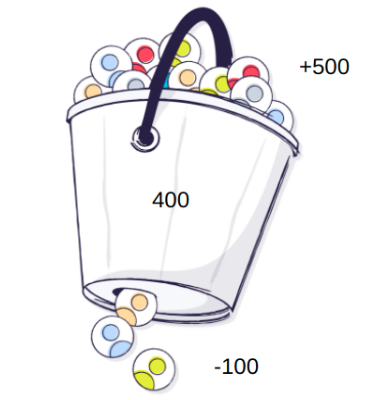
\includegraphics[width=0.8\linewidth]{churn1}
        \caption{SearX‌‌ gains ‌‌five ‌‌hundred‌‌ users‌‌ and‌ ‌loses‌ ‌one‌ ‌hundred‌ ‌users‌ ‌in‌ ‌the‌ ‌first‌‌ month‌ ‌the‌ ‌engine‌ ‌was‌ ‌launched.‌ ‌Since‌‌ there‌ ‌were‌‌ no‌‌ users‌‌ at‌‌ the‌‌ beginning‌‌ of‌‌ the‌‌ month,‌‌four‌‌ hundred‌‌ users‌‌ remained‌‌ by‌‌ the‌‌ end‌ ‌of‌ ‌the‌ ‌month.}
        \label{fig:churn1}
    \end{subfigure}%
    \hfill%
    \begin{subfigure}[t]{0.4\linewidth}
        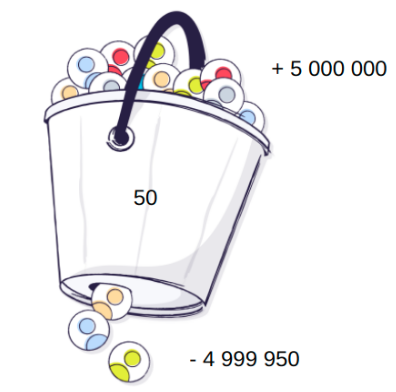
\includegraphics[width=0.8\linewidth]{churn2}
        \caption{‌‌‌SearX‌ ‌gains‌ ‌five‌ ‌million‌ ‌users‌‌ and‌‌ loses ‌‌all‌‌ users,‌‌except‌‌ for ‌‌fifty‌‌ users, ‌‌in‌‌ the‌ ‌first‌ ‌month‌ ‌the‌ ‌engine‌ ‌was‌ launched.‌‌ Since‌ ‌there‌ ‌were ‌‌no ‌‌users ‌‌at‌‌ the ‌‌beginning‌‌ of‌ ‌the‌ ‌month,‌ ‌fifty‌ ‌users‌ ‌remained‌ ‌by‌ ‌the‌‌ end‌ ‌of‌ ‌the‌ ‌month.}
        \label{fig:churn2}
    \end{subfigure}%
    \hfill%
    \caption{Churn scenarios.}
\end{figure}

There‌‌ is‌‌ a‌‌ term‌‌ used‌‌ to‌‌ describe‌‌ this‌‌ phenomenon‌‌ of‌‌ users‌‌ leaving‌‌ a‌‌ service, ‌‌which ‌‌is ‌‌known‌‌ as‌‌ customer‌ ‌churn.‌ \newpage

\subsection{Customer churn}

Mathematically‌ ‌speaking,‌ ‌the‌ ‌customer‌ ‌churn‌ ‌can‌ ‌be‌ ‌described‌ ‌as‌ ‌the‌ ‌coefficient‌ ‌between‌ ‌the‌‌
number‌ ‌of‌ ‌users‌ ‌that‌ ‌have‌ ‌left‌ ‌the‌ ‌service‌ ‌and‌ ‌all‌ ‌users‌ ‌for‌ ‌a‌ certain‌ ‌time‌ ‌period‌ ‌[21‌],‌ ‌as‌ ‌written‌‌
in‌ ‌the‌ ‌formula‌ ‌below:‌

\begin{equation}
    \text{Customer Churn Rate} = \frac{\text{Churned}}{\text{I}}
    \label{eq:customerchurnrate}
\end{equation}

Another‌ ‌way‌ ‌to‌ ‌write‌ ‌the‌ ‌formula‌ ‌is represented in \autoref{eq:customerchurnrate2}, where‌ ‌user‌ ‌retention‌ ‌is‌ ‌the‌ ‌average‌ ‌time‌ ‌someone‌ ‌is‌ ‌a‌ ‌user. 

\begin{equation}
    \text{Customer Churn Rate} = \frac{1}{\text{User Retention}}
    \label{eq:customerchurnrate2}
\end{equation}‌

On‌ ‌a‌ ‌side‌ ‌note,‌ ‌the‌ ‌customer‌ ‌churn‌ ‌rate‌ should not ‌be‌ ‌mistaken‌ ‌for‌ ‌the‌ ‌gamma‌ ‌parameter‌ ‌used‌‌ in‌ ‌the‌ ‌models.‌ ‌The‌ ‌gamma‌ ‌parameter‌ ‌can‌ ‌have‌ ‌a‌ ‌value‌ ‌bigger‌ ‌than‌ ‌1,‌ ‌while‌ ‌the‌ ‌value‌ ‌of‌ ‌churn‌‌ rate‌ ‌is‌ ‌in‌ ‌the‌ ‌range‌ ‌between‌ ‌0‌ ‌and‌ ‌1‌ ‌included.‌‌ ‌‌

\subsection{The many forms and shapes of churn}

More‌‌ often‌‌ than‌‌ not,‌‌companies‌‌ tend‌‌ to‌‌ determine‌‌ their‌‌ churn‌‌ in‌‌ a‌‌ way‌‌ that‌‌ gives‌‌ them‌‌ the‌‌ most‌‌ pleasant‌ ‌results.‌‌By‌‌ sharing‌‌ those‌‌ results‌‌ publicly,‌‌ they‌‌ can‌‌ stay‌‌ "ahead"‌‌ in‌‌ the‌‌ market.‌‌ This‌‌ is‌‌ possible‌‌ because‌‌ there‌‌ are‌‌ other‌‌ types‌‌ of‌‌ churn‌‌ that‌‌ go‌‌ beyond‌‌ the‌‌ customer‌‌ churn.‌‌ Therefore,‌‌ the‌‌ details‌‌ about‌‌ how‌‌ the‌‌ churn‌‌ was‌‌ calculated‌‌ can‌‌ be‌‌ hidden‌‌ in‌‌ a‌‌ way‌‌ that‌‌ can‌‌ easily‌‌ trick‌‌ the‌‌ public,‌ ‌especially‌ ‌those‌ ‌who‌ ‌are‌ ‌ignorant‌ ‌about‌ ‌the‌ ‌topic‌ [22].

When ‌‌a‌‌ company‌‌ mentions‌‌ their‌‌ churn‌‌ rate,‌‌without‌‌ any‌‌ further‌‌ details,‌‌ that‌‌ rate‌‌ should‌‌ not‌‌ be‌‌ taken‌ ‌with‌ ‌a‌ ‌dogmatic‌ ‌mindset.‌ ‌Instead,‌ ‌the‌ ‌following‌ ‌questions‌ ‌should‌ ‌have‌ ‌clear‌ ‌and‌‌ well-defined‌ ‌answers:‌

\begin{enumerate}
    \item Is‌ ‌it‌ ‌a‌ ‌customer‌ ‌churn‌ ‌or‌ ‌a‌ ‌revenue‌ ‌churn?‌‌
    \item Was‌ ‌the‌ ‌churn‌ ‌calculated‌ ‌for‌ ‌a‌ ‌week,‌ ‌month,‌ ‌year,‌ ‌or‌ ‌a‌ ‌different‌ ‌time‌ ‌range?‌
    \item Is‌ ‌it‌ ‌based‌ ‌on‌ ‌a‌ ‌gross‌ ‌churn‌ ‌or‌ ‌a‌ ‌net‌ ‌churn?‌ ‌
\end{enumerate}

Any‌ ‌company,‌ ‌including‌ ‌SearX,‌ ‌should‌ ‌be‌ ‌able‌ ‌to‌ ‌understand‌ ‌the ‌‌concepts ‌‌of ‌‌revenue ‌‌churn,‌‌ gross ‌‌churn‌‌ and‌‌ net ‌‌churn, ‌‌so‌‌ that‌‌ the‌‌ company ‌‌is ‌‌capable ‌‌of‌‌ answering‌‌ these‌‌ questions.‌‌ The‌‌ concept‌ ‌of‌ ‌customer‌ ‌churn‌ ‌has‌ ‌been‌ ‌previously‌ ‌explained,‌ ‌hence‌ ‌its‌ ‌exclusion.

Revenue ‌‌churn‌‌ is ‌‌similar ‌‌to‌‌ customer‌‌ churn,‌‌but ‌‌instead‌‌ of‌‌ focusing‌‌ on ‌‌the‌‌ users,‌‌ it ‌‌focuses‌‌ on‌‌ the‌ ‌revenue,‌ ‌as‌ ‌the‌ ‌name‌ ‌suggests‌ ‌[23‌].‌‌The‌‌ revenue‌‌ churn‌‌ can‌‌ be‌‌ either‌‌ calculated‌‌ monthly‌‌ (MRR‌ ‌-‌ ‌Monthly‌ ‌Recurring‌ ‌Revenue)‌ ‌or‌ ‌yearly‌ ‌(ARR‌ ‌-‌ ‌Annual‌ ‌Recurring‌ ‌Revenue).‌ ‌It‌ ‌can‌‌ be‌‌
determined‌ ‌by‌ ‌the‌ ‌following‌ ‌formula:‌ ‌

\begin{equation}
    \text{Revenue Churn} = \frac{\text{Net Revenue Lost frm Existing Customers in a Given Period}}{\text{Total Revenue at the Beginning of Period}}
    \label{eq:revenuechurn}
\end{equation}

As‌‌ for‌‌ the‌‌ gross‌‌ churn,‌ it‌‌ is‌‌ basically‌‌ the‌‌ type‌‌ of‌‌ churn‌‌ which‌‌ has‌‌ already‌‌ been‌‌ used‌‌ to‌‌ describe‌‌ the‌ ‌customer‌ ‌and‌ ‌revenue‌ ‌churn,‌ ‌that‌ ‌is,‌ ‌the‌ ‌amount‌ ‌of‌ ‌users‌ ‌or‌ ‌money‌ ‌lost‌ ‌during‌‌a‌‌certain‌‌ time‌ ‌period‌ ‌[24].‌

Finally,‌ ‌the‌ ‌concept‌ ‌of‌‌ net‌‌ churn‌‌ is‌‌ identical‌‌ to‌‌ gross‌‌ churn,‌‌ but‌‌ it‌‌ excludes‌‌ the‌‌ total‌‌ amount‌‌ of‌‌ revenue‌ ‌earned‌ ‌from‌ ‌plan‌ ‌upgrades,‌ ‌expansions‌ ‌and‌ ‌reactivations‌ [25]‌.

\subsection{Mechanisms that influence the popularity of SearX}

Mechanisms‌ ‌that‌ ‌can‌ ‌affect‌ ‌customer‌ ‌churn,‌ ‌as‌ ‌well‌ ‌as‌ ‌the‌ ‌number‌ ‌of‌ ‌new‌ ‌users,‌ ‌are‌ ‌the‌‌ following:‌ ‌marketing‌ ‌-‌ ‌trends,‌ ‌advertisement,‌ ‌influence‌ ‌from‌ ‌other‌ ‌users,‌ ‌and‌ ‌so‌‌on; ‌‌quality‌‌ of‌‌ service;‌ ‌user‌ ‌interface‌ ‌and‌ ‌user‌ ‌experience‌ ‌and‌ ‌innovation.‌

\section{Conclusion}

As‌ ‌a‌ ‌model‌ ‌gets‌ ‌progressively‌ ‌more‌ ‌complex,‌ ‌it‌ ‌tends‌ ‌to‌ ‌become‌ ‌more‌ ‌accurate,‌ ‌since‌ ‌the‌‌ model‌ ‌takes‌ ‌into ‌‌consideration‌‌ more‌‌ scenarios‌‌ and‌‌ situations,‌‌which‌‌ might‌‌ be‌‌ common‌‌ or‌‌ not.‌‌ This‌ ‌does not ‌mean‌‌ that‌‌ the‌‌ simpler,‌‌atomic‌‌ models‌‌ are not relevant‌‌ or‌‌ useful.‌‌ Depending‌‌ on‌‌ the‌‌ budget‌ ‌and‌‌ time‌‌ available ‌‌it‌‌ might‌‌ be‌‌ a‌‌ smarter‌‌ decision‌‌ to‌‌ create‌‌ a‌‌ simpler‌‌ but‌‌ less‌‌ accurate‌‌ model‌ ‌over‌ ‌a‌ ‌more‌ ‌accurate‌ ‌one.‌ ‌Overall,‌ ‌it‌ ‌is‌ ‌a‌ ‌matter‌ ‌of‌ ‌common‌ ‌sense‌ ‌when‌ ‌it‌ ‌comes‌ ‌to‌‌ choosing‌ ‌the‌ ‌best‌ ‌model‌ ‌to‌ ‌predict‌ ‌the‌ ‌popularity‌ ‌of‌‌SearX,‌‌or‌‌ the‌‌ best‌‌ model‌‌ to‌‌ predict‌‌ other‌‌ contexts,‌ for‌ ‌that‌ ‌matter.‌

On‌ ‌a‌ ‌personal‌ ‌opinion,‌ ‌this‌ ‌work‌ ‌was‌ ‌left‌ ‌with‌ ‌some‌ ‌unexplained‌ "black‌ ‌boxes",‌ ‌particularly‌‌ when‌ ‌it‌ ‌comes‌ ‌to‌ ‌the‌ ‌mechanisms‌ ‌that‌ ‌constitute‌ ‌the‌ ‌Gillespie‌ ‌algorithm‌ ‌and‌ ‌optimal‌ ‌control.‌‌ The‌ ‌fact‌ ‌that‌ ‌some‌ ‌details‌ ‌behind‌ ‌the‌ ‌modeling‌ ‌and‌ ‌implementation‌ ‌of‌ ‌these‌‌ algorithms ‌‌were‌‌ not‌ ‌fully‌ ‌understood,‌ ‌as‌ ‌well‌ ‌as‌ ‌the‌ ‌report‌ ‌size‌ ‌constraint,‌ ‌were‌ ‌the‌ ‌main‌ ‌reasons‌ ‌for‌ ‌this‌‌ occurrence.‌ ‌Structuring‌ ‌the‌ ‌thoughts‌ ‌into‌ ‌words‌ ‌was‌ ‌also‌ ‌harder‌ ‌than‌ ‌expected.‌

% \bibliography{references}

\end{document}